Damit in einem Projekt Veränderungen und Entwicklungen in Umwelten frühzeitig erkannt werden können, um richtig reagieren zu können, werden Umweltanalysen angefertigt. Hier werden die Umfelder nach verschiedenen Kriterien analysiert, die das Projekt auf eine gewisse Art beeinflussen. Das tatsächliche Ziel ist es, eine Übersicht über die Umwelten zu haben, um Handlungsempfehlungen ausgeben zu können. Im Marketing wird zwischen internen und externen Faktoren unterschieden. Die Einflussgröße der Umwelten werden mit \enquote{++}, \enquote{+}, \enquote{0}, \enquote{-} und \enquote{--} beschrieben, wobei \enquote{++} für sehr großen und \enquote{--} für sehr kleinen Einfluss steht. \cite[vgl.][]{Wikipedia:2023, Redaktion:2024}. \\
Die folgende Abbildung \ref{fig:umweltanalyse} beschreibt grob die um die Diplomarbeit herum existierenden Umwelten. Diese werden in der darunter liegenden Tabelle \ref{tab:umweltbeziehungen} nochmals aufgezählt und genauer geschildert.

\begin{figure}[H]
	\centering
	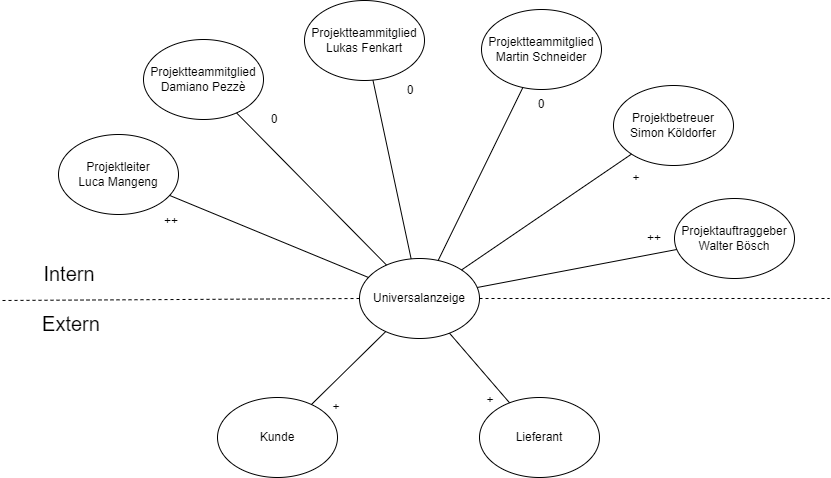
\includegraphics[width=15cm]{Bilder/pua.png}
	\caption{Projektumweltanalyse}
	\label{fig:umweltanalyse}
\end{figure}

\begin{longtable}{p{\dimexpr 0.20\textwidth-2\tabcolsep} | p{0.10\textwidth} | p{0.33\textwidth} | p{0.22\textwidth}}
	\caption{Projektumweltbeziehungen}
	\label{tab:umweltbeziehungen}
	\\ \toprule
	\textbf{Umwelten} & \textbf{Einfluss-größe} & \textbf{Risiko} & \textbf{Maßnahmen}
	\\ \midrule
	\endfirsthead
	\caption{Projektumweltbeziehungen (Fortsetzung)}
	\\ \toprule
	\textbf{Umwelten} & \textbf{Einfluss-größe} & \textbf{Risiko} & \textbf{Maßnahmen}
	\\ \midrule
	\endhead
	%
	\midrule
	\multicolumn{4}{r}{{Fortsetzung auf der nächsten Seite}} 
	\\ \bottomrule
	\endfoot
	%
	\bottomrule
	\endlastfoot
	Projektauftrag-geber & ++ & Unerwartete Änderungen in den Vertragsbedingungen & Engen Kontakt aufrechterhalten und klare Vertragsbedingungen definieren \\
	\midrule
	Projektbetreuer & + & Mangelnde Zusammenarbeit mit dem Projektteam könnte die Umsetzung und Überwachung des Projektes beeinträchtigen & Enge Zusammenarbeit mit dem Projektteam \\
	Projektleiter & ++ & Ungenaue Kommunikation der Projektziele und -anforderungen könnte zu Missverständnissen führen & Klare Kommunikation der Ziele und regelmäßige Statusberichte \\
	\midrule
	Projektteam-mitglieder & 0 & Arbeitsabläufe könnten durch interne Konflikte oder ineffiziente Prozesse beeinträchtigt werden & Effiziente Arbeitsabläufe sicherstellen und mögliche Konfliktslösungen aufbauen \\
	\midrule
	Kunde & + & kein Nutzen für den Kunden und es wird  kein Absatzmarkt gefunden & Anforderungen des Kunden verstehen und Kundenbedarf überprüfen \\
	\midrule
	Lieferant & + & Lieferverzögerungen oder Qualitätsprobleme & mehrere Lieferantenoptionen prüfen \\
\end{longtable}
